	%
%  untitled
%
%  Created by Julian Sackmann on 2012-02-06.
%  Copyright (c) 2012 __MyCompanyName__. All rights reserved.
%
\documentclass[]{article}

% Use utf-8 encoding for foreign characters
\usepackage[utf8]{inputenc}
\usepackage[spanish]{babel}

% Setup for fullpage use
\usepackage{fullpage}

% Uncomment some of the following if you use the features
%
% Running Headers and footers
%\usepackage{fancyhdr}

% Multipart figures
%\usepackage{subfigure}

% More symbols
\usepackage{amsmath}
\usepackage{amsthm}
\usepackage{amssymb}
\usepackage{latexsym}
\usepackage{amsthm}
\usepackage{dsfont}
%\usepackage{texsync}

% Surround parts of graphics with box
\usepackage{boxedminipage}

% Package for including code in the document
\usepackage{listings}

% If you want to generate a toc for each chapter (use with book)
\usepackage{minitoc}

% This is now the recommended way for checking for PDFLaTeX:
\usepackage{ifpdf}

% Más paquetes
\usepackage{cancel}
%\newif\ifpdf
%\ifx\pdfoutput\undefined
%\pdffalse % we are not running PDFLaTeX
%\else
%\pdfoutput=1 % we are running PDFLaTeX
%\pdftrue
%\fi

\ifpdf
\usepackage[pdftex]{graphicx}
\else
\usepackage{graphicx}
\fi
\title{Un (no tan corto) resumen de Análisis I}
\author{ Julián Sackmann }

\date{10/04/2012}

\newtheorem{teo}{Teorema}
\newtheorem{defi}[teo]{Definición}
\newtheorem{lem}[teo]{Lema}
\newtheorem{prop}[teo]{Proposición}
\newtheorem{cor}[teo]{Corolario}
\newtheorem{obs}[teo]{Observación}


\def\N{\mathbb{N}}
\def\R{\mathbb{R}}
\def\Z{\mathbb{Z}}
\def\Q{\mathbb{Q}}
\def\e{\varepsilon}
\def\d{\delta}

\newcommand{\ip}[2]{\langle #1,#2 \rangle}
\newcommand{\dprim}[2]{\frac{\partial #1}{\partial #2}}
\newcommand{\dseg}[3]{\frac{\partial^2 #1}{\partial #2\ \partial #3}}
\newcommand{\dter}[4]{\frac{\partial^3 #1}{\partial #2\ \partial #3\ \partial #4}}
\newcommand{\zum}[2]{\sum_{#1}^{#2}}
\newcommand{\integral}[4]{\int_{#1}^{#2} \! #3 \, \mathrm{d}#4}
\newcommand{\intres}[3]{\int_{#1}^{#2} \! #3}
\newcommand{\dintegral}[7]{\int_{#1}^{#2} \! \int_{#3}^{#4} \! #5 \, \mathrm{d}#6 \, \mathrm{d}#7}
\newcommand{\dintres}[5]{\int_{#1}^{#2} \! \int_{#3}^{#4} \! #5}


%\newenvironment{proof}{{\bfseries Demostración. \rm}}{\qed}

\begin{document}

\ifpdf
\DeclareGraphicsExtensions{.pdf, .jpg, .tif}
\else
\DeclareGraphicsExtensions{.eps, .jpg}
\fi

\maketitle

\section{Introducción}
\begin{prop}[Principio de Arquimedianeidad]
	Si $x$ es un número real, entonces existe $n \in \N$ tal que $n > x$.
\begin{proof}
	Sean $x \in \R$ y $X = \{k \in \N : k \leq x \}$. Si $X = \emptyset$, entonces el principio vale pues $1 > x$ y se puede considerar $n = 1$. Si $x \neq \emptyset$, como está acotado superiormente (por $x$), tiene un supremo $s =$ sup$ X \in \R$. Necesariamente debe existir $k_0 \in X \in \N$ tal que $s - 1 < k_0$ (pues $s - 1$ no es cota superior). Tomando $n = k_0 + 1$ se tiene $n \in \N$ y $n > s$. O sea $n \not\in X$ lo que implica que $n > x$.
\end{proof}
\end{prop}

\begin{prop}[Equivalencia de Supremo]
	$s$ es el supremo de $A$ si y sólo si:
	\begin{itemize}
		\item $s \geq a$ para todo $a \in A$
		\item dado $\e > 0$ existe $a \in A$ tal que $s - \e < a$
	\end{itemize}
\begin{proof}
	~\newline
	$\Rightarrow)$ El primer ítem es trivial. Por otro lado, dado $\e > 0$, se tienen $s - \e < s$, por lo que $s - \e$ no es cota superior de $A$. O sea, existe $a \in A$ tal que $s-\e<a$, lo que prueba el segundo ítem.\newline
	~\newline
	$\Leftarrow)$ Es necesario probar que $s$ es la cota superior más chica. Sea $s'$ una cota superior más chica que $s$ (O sea $s' < s$) y sea $\e=s-s'>0$. Esto es absurdo porque contradice la hipótesis de que para cualquier $\e>0$, existe $a\in A$ tal que $s-\e<a$.
\end{proof}
\end{prop}

\newpage
\section{Sucesiones}
\begin{prop}
	Si $s = sup\ A$ entonces existe una sucesión creciente ${a_n} \in A$ tal que $a_n \rightarrow s$. Si $s \not\in A$, se puede elegir $a_n$ estrictamente creciente.
\begin{proof}
	Si $s \in A$, basta tomar $a_n = s$ la sucesión constante (que, por definición es creciente). Si no, tomamos algún elemento $\overline{a_1} \in A$, y ponemos $a_1 := \overline{a_1}$. 
	
	Ahora consideremos $\overline{a_2} = \frac{a_1 + s}{2}$. Vale que $\overline{a_2} < s$. Entonces existe $a_2 \in A$ tal que $\overline{a_2} < a_2 < s$. Si no existiera, $\overline{a_2}$ sería cota superior de $A$, lo cual es imposible pues $\overline{a_2} < s.$ Así vamos definiendo $\overline{a_n}$ como el promedio $\frac{a_{n-1}+s}{2}$, y tomamos como $a_n$ cualquier elemento de A que está entre $\overline{a_n}$ y $s$. La sucesión $a_n$ verifica ser creciente (pues $a_n > \overline{a_n} > a_n-1$) y vale que
	
	\begin{center}
		$0 < a_1 < a_2 < a_3 < \hdots < a_n$
	\end{center}
	\begin{center}
		$0 < s-a_n < \frac{s-a_{n-1}}{2} < \hdots < \frac{s-a_1}{2^{n-1}}$
	\end{center}
	O sea que $\displaystyle \lim_{n \to \infty} a_n = s$.
\end{proof}
\end{prop}

\begin{prop}
	Toda sucesión $\{a_n\} \subseteq \R$ tiene una subsucesión $\{a_{n_k}\}$ monótona.
	\begin{proof}
		Se dice que un término $a_i$ es \textbf{dominante} si verifica que $\forall k \geq i$ vale que $a_k \leq a_i$. Ahora se deben considerar dos casos: que haya finitos o infinitos términos dominantes:
		\begin{itemize}
			\item \textbf{Infinitos términos dominantes:} Sean $n_1 < n_2 < n_3, \hdots$ los índices tales que $a_{n_i}$ es un término dominante. La subsucesión $\{a_{n_i}\}$, por tener todos términos dominantes, verifica que: 
			\begin{center}
				$a_{n_1} \geq a_{n_2} \geq a_{n_3} \geq \hdots $
			\end{center}
			Con lo que hemos construido una subsucesión decreciente y, por ende, monótona.
			\item \textbf{Finitos términos dominantes:} Sea $a_u$ el último término dominante. Consideremos $a_{n_1} := a_{u+1}$ o sea, el primer término después del último término dominante (si no hay ningún término dominante tomamos $n_1 = 1$). Como $a_{n_1}$ no es dominante, sabemos que existe $n_2$ tal que $a_{n_2} > a_{n_1}$. A su vez, como $a_{n_2}$ tampoco es dominante (pues $n_2 > u$ y $u$ era el último término dominante), tiene que existir un $n_3$ tal que $a_{n_3}  > a_{n_2} > a_{n_1}$. De esa forma, siempre podemos hallar $n_k$ tal que
			\begin{center}
				$a_{n_k} > a_{n_{k-1}} > \hdots > a_{n_2} > a_{n_1}$
			\end{center}
			Con esto, hemos construido una subsucesión creciente y, por ende, monótona.
		\end{itemize}
	\end{proof}
\end{prop}

\begin{prop}[Bolzano-Weierstrass]
	Toda sucesión $\{a_n\} \subseteq \R$ acotada tiene una subsucesión $\{a_{n_k}\}$ convergente.
	\begin{proof}
		Sea $\{a_{n_k}\}$ una subsucesión monótona de $\{a_{n}\}$ (que se puede extraer por la proposición anterior). Como $\{a_{n_k}\}$ es una subsucesión monótona y acotada (por ser $\{a_{n}\}$ acotada), contiene una subsucesión $\{a_{n_{k_j}}\} = \{a_{n_{k'}}\}$ convergente.
	\end{proof}
\end{prop}

\begin{prop}[Cauchy]
	Sea $a_k$ una sucesión de números reales y sea $\displaystyle S_n = \sum_{k=0}^{n}a_k$ la sucesión de sumas parciales. Entonces

	~\newline
	$1.$ $a_k\to 0$ no implica que la serie converge.
	
	~\newline
	$2.$ Si la serie converge, entonces $a_k \to 0$.
	
	~\newline
	$3.$ Una serie de términos positivos $a_k \geq1 0$ es convergente si y sólo si sus sumas parciales están acotadas, pues en este caso, $S_n$ es una sucesión creciente de números reales.
\end{prop}

\newpage
\section{Conjuntos}
\begin{prop}
	Un conjunto $C \subset \R^n$ es cerrado si y sólo si su complemento $C^c$ es abierto.
	\begin{proof}
		~\newline
		$\Rightarrow$) Veamos que $C^c$ es abierto, o sea, que $\forall p \in C^c,\ p$ es interior. Sea $p \in C^c$ no interior. Entonces, $\forall k \in \N$ se tiene $B_{\frac{1}{k}}(P) \not\subseteq C^c$, o sea, existe $P_k \in C^{c^c} = C$ tal que $P_k \in B_{\frac{1}{k}}(P)$. Observemos que $P_k \rightarrow P$ (pues $||P_k - P|| < \frac{1}{k}$). 
		Hemos llegado a una contradicción pues $P_k \in C$, $P \not\in C$ y, por hipótesis, $C$ es cerrado.

		~\newline
		$\Leftarrow$) Consideremos $\{P_k\} \subseteq C$ una sucesión de puntos de $C$ con límite $P \in \R^n$. Queremos ver que $P \in C$ o, equivalentemente, $P \not\in C^c$. Si se diera lo segundo, existiría $r > 0$ tal que $B_r(P) \subset C^c$. Consideremos $k \in \N$ tal que $||P_k - P|| < r$. Entonces, tendríamos que $P_k \in B_r(P) \subset C^c$, lo que es imposible pues $P_k \in C$. Luego, $P \in C$, lo que demuestra que $C$ es cerrado.
	\end{proof}
\end{prop}

\begin{prop}
	La clausura $\overline{C}$ es un conjunto cerrado.
	\begin{proof}
		Sea $P \in \overline{C}^c$ un punto cualquiera. Entonces afirmo que existe $r > 0$ tal que $B_r(P) \bigcap C = \emptyset$ (de lo contrario, uno podría fabricar una sucesión $X_k$ de puntos de C tal que $X_k \rightarrow P$, lo que diría que $P \in \overline{C}$, contradiciendo que $P \in \overline{C}^c$). 
		
		Esto implica que $P$ es un punto interior de $\overline{C}^c$ y, como no impusimos ninguna restricción sobre $P$, vale que $\forall P \in \overline{C}^c$, $P$ es interior. Esto implica que $\overline{C}^c$ es un conjunto abierto, demostrando que $\overline{C}$ es un conjunto cerrado.
	\end{proof}
\end{prop}

\newpage
\section{Funciones}
\begin{prop}
	Sea $F:A \subset \R^n \to \R^m$. Sean $P \in \overline{A}$ y $L \in \R^m$. Las siguientes afirmaciones son equivalentes:
	\begin{itemize}
		\item $1)$ $\displaystyle \lim_{X \to P} F(X) = L$.
		\item $2)$ Para \textbf{toda} sucesión de puntos $P_k \rightarrow P$, se tiene que $\displaystyle \lim_{n \to \infty} F(P_k) = L$.
	\end{itemize}
	\begin{proof}
		~\newline	
		$(1) \Rightarrow (2)$ Sea $P_k$ una sucesión de puntos de $A$ que tiende a $P$. Entonces por la definición del límite de función, dado $\e > 0$ existe $\delta > 0$ tal que
		\begin{center}
			$0 < ||X-P|| < \delta$ y $X \in A \Rightarrow ||F(X)-L||<\e$.
		\end{center}
		Si tomamos $k_0 \in \N$ tal que $k \geq k_0$ implique $||P_k - P|| < \d$, lo anterior nos garantiza que $||F(P_k)-L|| < \e $. O sea $F(P_k) \to L$ de acuerdo a la definición de límite de sucesiones, aplicado a la sucesión $Q_k=F(P_k)$.
		
		~\newline	
		$(1) \Leftarrow (2)$ Negar que $\displaystyle \lim_{X \to P} F(X) = L$ equivale a decir que existe $\e > 0$ tal que para todo $\d > 0$ existe $X \in A$ con $0<||X-P||<\d$ y $||F(X)-L|| \geq \e$. Tomemos $\d = \frac{1}{k}$, con $k \in \N$, y sea $P_k$ el punto correspondiente. Vemos que $P_k \rightarrow P$ pero, por otro lado, $||F(P_k) - L|| \geq \e$, con lo cual $F(P_k) \nrightarrow	 L$, contradiciendo la hipótesis.
	\end{proof}
\end{prop}

\begin{prop}[Bolzano]
	Si $f:[a,b] \to \R$ es continua y $f(a).f(b) < 0$, entonces existe $c \in (a,b)$ tal que $f(c) = 0$.
	\begin{proof}
		Supongamos $f(a) > 0$ y $f(b) < 0$. Sea $A = \{x\in [a,b]: f(x) > 0\} \neq \emptyset$ (pues $a \in A$). A tiene supremo por estar acotado superiormente (pues $A \subset [a,b]$) y sea $s = $ sup$\ A$. Afirmo entonces que $f(s) = 0$. Si no fuera así, debería ser $f(s)>0$ o $f(s)<0$.
		\begin{itemize}
	 		\item $f(s) > 0$. Debería existir un entorno $(s-\e , s+\e)$ al rededor de $s$ tal que para todo $x$ en el entorno $f(x) > 0$. Sea un punto $x_0 \in (s,s+\e)$. Este $x_0$ verifica que $x_0 \in A$ (porque $f(x_0) > 0$ y $x_0 < b$) y $x_0 > s$ lo cual es absurdo pues $s$ es el supremo de $A$.
			\item $f(s) < 0$. Se demuestra en forma análoga al caso anterior que es absurdo.
		\end{itemize}
		Ergo, la única opción que queda es que $f(s) = 0$, que es lo que queríamos demostrar.
	\end{proof}

	\begin{proof}[Demostración alternativa]
		Supongamos $f(a) > 0$ y $f(b) < 0$. Sea $A = \{x\in [a,b]: f(x) > 0\} \neq \emptyset$ (pues $a \in A$). A tiene supremo por estar acotado superiormente (pues $A \subset [a,b]$) y sea $s = $ sup$\ A$. Entonces existe una sucesión creciente $\{a_n\}$ de puntos de $A$ que tiende a $s \in [a,b]$.
		
		Como $f(a_n) > 0$ (pues $a_n \in A$) entonces $f(s) \geq 0$. Afirmo entonces que $f(s) = 0$. Si no fuera así, debería ser $f(s)>0$ y eso es imposible porque debería existir un entorno $(s-\e , s+\e)$ al rededor de $s$ tal que $f(x) > 0$. Pero, como $s < b$, podemos tomar $x_0 \in [a,b]$ tal que $x_0 \in (s,s+\e)$. Este $x_0 \in A$ y es mayor que el supremo, lo que es absurdo. O sea $f(s) = 0$.
	\end{proof}
\end{prop}

\begin{prop}[Weiestrass]
	Sean $A \subset \R^n$ compacto y $f:A \to \R$ continua en $A$. Entonces vale que:
	\begin{itemize}
		\item $1)$ Existen $m,M \in \R$ tales que $m \leq f(X) \leq M$ para todo $X \in A$. 
		\item $2)$ Existen $P_m, P_M \in A$ tales que $f(P_m) = $ min$\{f(X):X \in A\}$ y $f(P_M) = $ max$\{f(X):X \in A\}$. O sea, $f$ alcanza su máximo y mínimo en A.
	\end{itemize}
	\begin{proof}
		~\newline
		$1)$ Supongamos que $f$ no es acotada, o sea, que no existe $M \in \R$ tal que $f(X) \leq M$. Entonces debe existir una sucesión de puntos $\{X_k\} \in A$ tal que $f(X_k) \geq k$ para todo $k \in \N$. Como $A$ es cerrado y acotado, $\{X_k\}$ necesariamente tiene una subsucesión $\{X_{k_j}\}$ que converge a $P \in A$. (Esto es porque toda sucesión en un conjunto acotado tiene límite en la clausura del conjunto. Como, en este caso $A$ es cerrado, su clausura coincide consigo mismo).\newline
		Sin embargo, como $f(X_k) \geq k$ y $f$ es continua, es imposible que exista $\{X_{k_j}\}$ convergente a $P$.\newline 
		~\newline
		$2)$ Por lo anterior, vale que $Im(f) \subseteq [m,M]$, o sea, es un conjunto acotado de $\R$. Sea $s = sup(Im(f))$. Queremos ver que en realidad $s$ es un máximo, o sea, que existe $P_M \in A$ tal que $f(P_M) = s$.
		Consideremos la sucesión $\{X_k\} \in A$ que, aplicándole la función $f$, tienda al supremo. Tenemos entonces una sucesión $\{X_k\} \in A$ tal que $\displaystyle \lim_{k \to \infty} f(X_k) = s$. \newline
		Ahora, de $\{X_k\}$ extraemos una subsucesión $\{X_{k_j}\}$ convergente y llamamos a su límite $P_M$ (que, por ser $\{X_k\}$ una sucesión de $A$ y este ser cerrado, $P_M \in A$). Como $f$ es continua $\displaystyle f(P_M) = \lim_{k \to \infty} f(X_k) = s$.
	\end{proof}
\end{prop}

\begin{prop}[Heine-Cantor]
	Continua en un compacto implica uniformemente continua. O sea, sea $F:A\subseteq R^n \to R^m$ continua con $A$ compacto. Entonces, vale que $F$ es uniformemente continua.
	\begin{proof}
		Supongamos que $f$ es continua pero no \textit{uniformemente} continua. Entonces, debe existir $\e_0 > 0$ tal que para todo $\d > 0$, existan $x,y \in A$ que verifiquen que $||F(x) - F(y)|| \geq \e_0$.\newline
		
		Consideremos dos sucesiones $\{X_k\}, \{Y_k\} \in A$ tales que $||X_k - Y_k|| < \frac{1}{k}$. Por lo anteriormente dicho, debe valer que $||F(X_k) - F(Y_k)|| \geq \e_0$. Como $A$ es compacto, deben existir dos subsucesiones $\{X_{k_j}\}, \{Y_{k_j}\}$ convergentes a $X_0$ e $Y_0$ respectivamente. Consideremos entonces
		\begin{center} 
			$||Y_{k_j} - X_0|| = ||Y_{k_j} - X_{k_j} + X_{k_j} - X_0|| \leq ||Y_{k_j} - X_{k_j}|| + ||X_{k_j} - X_0|| < \frac{1}{k_j} + ||X_{k_j} - X_0||$
		\end{center}
		O sea que ambas sucesiones convergen al mismo valor $X_0 = Y_0$. Sin embargo, esto no es posible pues contradice que $||F(X_k) - F(Y_k)|| \geq \e_0$.
	\end{proof}
\end{prop}

\begin{prop}
	Sea $G:[a,b)\to\R$ una función creciente ($b$ puede ser $+\infty$). Entonces existe el límite $\displaystyle \lim_{x\to b^-}G(x)$. Además, este límite es finito si y sólo si $G$ es acotada superiormente.
	\begin{proof}
		Sea $l=$ sup$\{G(x):x\in[a,b)\}$. Por definición de supremo, dado $\e>0$, existe $x_0 \in [a,b)$ tal que $l-G(x_0) < \e$. Si $|b-x| = b - x < \delta = b-x_0$, entonces $x\leq x_0$ y $G$ es creciente $G(x) \leq G(x_0)$. Entonces
		\begin{center}
			$l-G(x) \leq l-G(x_0) < \e$
		\end{center}
		lo que prueba que el límite existe y coincide con el supremo. En particular el límite es finito si y sólo si $G$ es acotada.
		Entonces, $\displaystyle l=\lim_{x\to b^-}G(x)$
	\end{proof}
\end{prop}

\newpage
\section{Diferenciación}
\begin{prop}[Diferenciable $\Rightarrow$ Continua]
	Sea $f:A \subset \R^n \to R$, $P \in A^o$. Si $f$ es \textbf{diferenciable} en $P$, entonces $f$ es \textbf{continua} en $P$.
	\begin{proof}
		Consideremos
		\begin{eqnarray*}
			& |f(X) - f(P)| & \leq |f(X) - f(P) - Df_p(X-P) + Df_p(X-P)| \\
			& & \leq |f(X) - f(P) - Df_p(X-P)| + |Df_p(X-P)| \\
			& & \leq |f(X) - f(P) - Df_p(X-P)| + ||\nabla f_p ||\ ||(X-P)||
		\end{eqnarray*}
		El último término sale por la desigualdad de Cauchy-Schwarz
		\begin{center}
			$|Df_p(X)| = |\ip{\nabla f_p}{X}| \leq ||\nabla f_p||\ ||X||$
		\end{center}
		
		Dividiendo y multiplicando por $||X-P||$ el primer sumando obtenemos:
		\begin{center}
			$|f(X)-f(P)|\leq \displaystyle \frac{|f(X)-f(P)-Df_p(X-P)|}{||X-P||}\ ||X-P||+||\nabla f_p||\ ||X-P|| \leq 0$
		\end{center}
		El primer sumando de la derecha tiende a cero cuando $X\to P$ por ser $f$ diferenciable en $P$. El segundo trivialmente también tiende a cero, con lo cual obtenemos que $\displaystyle \lim_{X\to P} f(X) = f(P)$ o, equivalentemente, $f$ es continua en $P$.
	\end{proof}
\end{prop}

\begin{prop}[Unicidad del Diferencial]
	Sea $f:A\subset \R^n \to R$, $P \in A^o$. Si existe una transformación lineal $T_p:\R^n \to \R$ tal que 
	\begin{equation}\label{DIFER}
		\displaystyle \lim_{X\to P} \frac{|f(X)-f(P)-T_p(X-P)|}{||X-P||} = 0
	\end{equation}
	Entonces\newline
	$1)$ Existen todas las derivadas direccionales de $f$ en $P$ y vale que
	\begin{center}
		$\displaystyle \frac{\partial f}{\partial V}(P) = T_p(V)$ para todo $V\in \R^n$, $||V||=1$
	\end{center}
	~\newline
	$2)$ En particular, existen todas las derivadas parciales de $f$, se tiene $f_{x_i}(P)=T_P(E_i)$ y la transformación $T_P$ es única.
	~\newline
	$3)$ Se tiene $T_P(X) = Df_P(X) = \ip{\nabla f_P}{X}$ para todo $X\in \R^n$, y $f$ es diferenciable en $P$. En particular, si $||V||=1$,
	\begin{center}
		$\displaystyle \frac{\partial f}{\partial V}(P) = \ip{\nabla f_P}{V} = Df_P(V)$
	\end{center}
	\begin{proof}
		~\newline
		$1)$ Sea $V\in \R^n$ tal que $||V||=1$. Como asumimos que existe el límite \eqref{DIFER}, también existe compuesto con cualquier curva que tenga límite $P$. En particular, si ponemos $X = P + tV$ (con $t$ suficientemente chico para que $X\in A$), vale que $X-P = tV$. Tomando módulo, $||X-P|| = |t|$, lo que implica que
		\begin{center}
			$\displaystyle 0 = \lim_{t\to 0} \frac{|f(P+tV) - f(P) - T_P(P+tV-P)|}{|t|} = \lim_{t \to 0} |\frac{f(P+tV) - f(P)}{t}-T_P(V)|$
		\end{center}
		~\newline
		Esto prueba que $f_V(P) = \displaystyle \lim_{t\to 0} \frac{f(P+tV)-f(P)}{t} = T_P(V)$. Como $V$ puede ser igual a $E_i$, también prueba que existen todas las derivadas parciales. \newline
		
		Además, como $T_P(E_i) = f_{x_i}(P)$ vale para toda $E_i$ y una transformación lineal queda determinada por su valor en una base de $\R^n$, se deduce que $T_P(X) = \ip{\nabla f_P}{X}$.\newline
		
		Supongamos que existe otra transformación $T'_P$ que verifique la condición del límite. Entonces, también debe cumplir que $T'_P(X) = \ip{\nabla f_P}{X} = T_P(X)$.\newline
		
	\end{proof}
\end{prop}

\begin{prop}
	Sea $f:A\subseteq \R^n \to \R$ y $P \in A$. El gradiente ($\nabla f_P$) es la dirección de mayor crecimiento de $f$ en $P$.
	\begin{proof}
		Sea $V$ de norma unitaria.
		\begin{center}
			$f_V(P) = \ip{\nabla f_P}{V} \leq |\ip{\nabla f_P}{V}| \leq ||\nabla f_P||\ ||V|| = ||\nabla f_P||$
		\end{center}
		Esto demuestra que la derivada direccional a lo sumo vale $||\nabla f_P||$. Por otro lado, si consideramos la dirección del gradiente normalizada poniendo $V_P = \frac{\nabla f_P}{||\nabla f_P||}$, se tiene:
		\begin{center}
			$f_{V_P} = \ip{\nabla f_P}{V_P} = \ip{\nabla f_P}{\frac{\nabla f_P}{||\nabla f_P||}} = ||\nabla f_P||$
		\end{center}
	\end{proof}
\end{prop}

\begin{teo}[Fermat]
	Si $f:[a,b]\to \R$ es derivable en $c\in (a,b)$ y $c$ es un extremo local de $f$, entonces $f'(c)=0$.
	\begin{proof}
		Supongamos que $c$ es máximo local de $f$. Por definición, esto significa que existe $\e > 0$ tal que si $x \in (c-\e,c+\e)$ entonces $f(x) \leq f(c)$. Calculemos $f'(c)$ por definición, usando límites laterales:
		\begin{center}
			$\displaystyle f'(c) = \lim_{x\to 0^-} \frac{f(c+h)-f(c)}{h} \geq 0$
		\end{center}
		Esto se debe a que $h<0$ (pues tiende a $0$ por izquierda) y $f(c+h) - f(c) \leq 0$ (pues $c$ es máximo local por hipótesis).\newline
		~\newline
		Análogamente considerando el límite por derecha tenemos que:
		\begin{center}
			$\displaystyle f'(c) = \lim_{x\to 0^+} \frac{f(c+h)-f(c)}{h} \leq 0$
		\end{center}
		Juntando ambas ecuaciones, debe valer que  $0\leq f'(c) \leq 0$, lo que implica $f'(c) = 0$
	\end{proof}
\end{teo}

\begin{teo}[Rolle]
	Si $f:[a,b]\to \R$ es continua en $[a,b]$ y derivable en $(a,b)$ y además $f(a) = f(b)$, entonces existe $c\in (a,b)$ tal que $f'(c)=0$.
	\begin{proof}
		Si $f$ es continua en $[a,b]$ y este último conjunto es compacto, $f$ alcanza su máximo y mínimo en $[a,b]$. Separemos en dos casos:
		\begin{itemize}
			\item $ max = min$. Si este es el caso, la función es la función constante y tomando cualquier $c\in (a,b)$ vale que $f'(c)=0$.\newline
			\item $ max \neq min$. Como $f(a) = f(b)$, puede ser que $f(a) = f(b) = max$ o $f(a) = f(b)=min$ (o ninguna de las dos). Pero necesariamente va a existir $c\in (a,b)$ tal que $c$ es máximo o mínimo; o sea $c$ es extremo local. Por el teorema de \textit{Fermat}, $f'(c)=0$
		\end{itemize}
	\end{proof}
\end{teo}

\begin{teo}[Lagrange]
	Si $f:[a,b]\to \R$ es continua en $[a,b]$ y derivable en $(a,b)$ entonces existe $c\in (a,b)$ tal que 
	\begin{center}
		$\displaystyle f'(c) = \frac{f(b)-f(a)}{b-a}$
	\end{center}
	\begin{proof}
		Sea la función $L(x)$ la recta que pasa por los puntos $(a,f(a))$ y $(b,f(b))$. O sea,
		\begin{center}
			$\displaystyle L(x) = (x-a)\frac{f(b)-f(a)}{b-a} + f(a)$
		\end{center}
		Consideremos la función auxiliar $g(x) = f(x) - L(x)$. Dado que $L(a) = f(a)$ y $L(b) = f(b)$, vale que $g(a) = g(b) = 0$. Además, por álgebra de funciones continuas y derivables, vale que $g$ es continua en $[a,b]$ y derivable en $(a,b)$. Entonces $g$ cumple las hipótesis del teorema de Rolle, lo que nos permite afirmar que existe $c\in (a,b)$ tal que $g'(c)=0$.\newline
		~\newline
		Sea $m$ la pendiente de la recta $L$. Entonces, tenemos que
		\begin{center}
			$0 = g'(c) = f'(c) - L'(c) = f'(c) - \displaystyle \frac{f(b)-f(a)}{b-a}$.
		\end{center}
		Reagrupando apropiadamente, tenemos que $\displaystyle f'(c) = \frac{f(b)-f(a)}{b-a}$
	\end{proof}
\end{teo}

\begin{teo}[Cauchy]
	Si $f,g:[a,b]\to \R$ son continuas en $[a,b]$ y derivables en $(a,b)$, entonces existe $c\in (a,b)$ tal que 
	\begin{center}
		$f'(c)(g(b)-g(a)) = g'(c)(f(b)-f(a))$
	\end{center}
	\begin{proof}
		Consideremos la función auxiliar 
		\begin{center}
			$h(x) = (f(x)-f(a))(g(b)-g(a))\ -\ (g(x)-g(a))(f(b)-f(a))$
		\end{center}
		Dado que $h(a)=h(b)=0$ y, por construcción, es continua en $[a,b]$ y derivable en $(a,b)$. Consecuentemente $h$ cumple las hipótesis del teorema de Rolle. O sea existe $c\in (a,b)$ tal que $h'(c) = 0$. Pero, por otra parte, vale que
		\begin{center}
			$0 = h'(c) = f'(c)(g(b)-g(a)) - g'(c)(f(b)-f(a))$
		\end{center}
		Despejando apropiadamente se obtiene la tesis del teorema.
	\end{proof}
\end{teo}

\begin{obs}
	Sea $F(u,v) = (f_1(u,v),f_2(u,v),f_3(u,v))$. Entonces, la fórmula de la derivada parcial respecto a la primer coordenada de la composición queda escrita de la siguiente manera:
	\begin{center}
		$\displaystyle \frac{\partial (g \circ F)}{\partial u} = \frac{\partial g}{\partial f_1}\frac{\partial f_1}{\partial u} + \frac{\partial g}{\partial f_2}\frac{\partial f_2}{\partial u} + \frac{\partial g}{\partial f_3}\frac{\partial f_3}{\partial u}$
	\end{center}
\end{obs}
~\newline

\begin{teo}[Lagrange en $\R^n$]
	Sea $f:A\subseteq \R^n\to \R$ diferenciable con $A$ \textbf{convexo} (o sea, para todo par de puntos del conjunto el segmento que los une está totalmente contenido en el conjunto). Entonces, para todo $Q,R\in A$, existe $P_0$ en el segmento que une $Q$ con $R$ tal que
	\begin{center}
		$f(Q)-f(R) = \ip{D_f(P_0)}{Q-R}$
	\end{center}
	\begin{proof}
		Consideremos la parametrización del segmento que une $Q$ con $R$, $\alpha(t) = R+t(Q-R)$. Entonces, $h(t) = f \circ \alpha(t)$ está definida y es continua en $[0,1]$ y es derivable en $(0,1)$ (por ser composición de continuas/diferenciables). Entonces, por el teorema de \textit{Lagrange} en una variable, existe $c\in (0,1)$ tal que $h(1) - h(0) = h'(c)$. Pero, por regla de la cadena, $h'(c) = Df_{\alpha(c)}\alpha'(c)^t = Df_{g'(c)}(Q-R)^t = \ip{D_f(\alpha(c))}{Q-R}$. Llamando $P_0$ a $\alpha(c)$ obtenemos la tesis.
	\end{proof}
\end{teo}

\begin{prop}
	Si $G:B_r(P) \subset \R^n \to \R^n$ es diferenciable y $||D_GQ||_{\infty} \leq M$ para todo $Q\in B_r(P)$, entonces se tiene que $||G(X)-G(Y)|| \leq M||X-Y||$ para todo $X,Y\in B_r(P)$
	\begin{proof}
		Si $G(X)=G(Y)$, entonces $0 \leq M||X-Y||$ es trivial. Supongamos $G(X)\neq G(Y)$. Consideremos el segmento que une $X$ con $Y$, o sea el segmento $g(t)=Y+t(X-Y)$. Pongamos la función auxiliar:
		\begin{center}
			$h(t) = \ip{G\circ g(t)}{G(X)-G(Y)}$
		\end{center}
		\begin{center}
			$h'(t) = \ip{DG_{g(t)}g'(t)}{G(X)-G(Y)}$
		\end{center}
		$h'(t)$ verifica las hipótesis del teorema de Lagrange, lo que nos permite afirmar que existe $c\in (0,1)$ tal que 
		\begin{center}
			$h(1)-h(0) = h'(c)(1-0)$
		\end{center}
		Reemplazando por la definición de $h$, esto nos lleva a la expresión:
		\begin{center}
			$\ip{G(X)-G(Y)}{G(X)-G(Y)} = \ip{DG_{Y+c(X-Y)(X-Y)}}{G(X)-G(Y)}$
			$||G(X)-G(Y)||^2 \leq ||DG_{Y+c(X-Y)}(X-Y)||_{\infty}||G(X)-G(Y)|| \leq M||X-Y||\ ||G(X)-G(Y)||$
		\end{center} 
		Como supusimos $G(X)\neq G(Y)$, entonces $||G(X)-G(Y)||\neq 0$, con lo cual podemos dividir ambos miembros por ese término, demostrando la afirmación buscada.
	\end{proof}
\end{prop}

\newpage
\section{Implícita e Inversa}
\begin{obs}
	Si $F$ es diferenciable e inversible, y su inversa también es diferenciable, entonces por regla de la cadena aplicada a $F^{-1}(F(X))$ vale que
	\begin{center}
		$DF^{-1}_{F(X)}DF_X=Id$
	\end{center}
	Donde $Id$ es la transformación identidad de $\R^n$. De aquí se deduce que la diferencial de la inversa es la inversa de la diferencial de $F$, o sea:
	\begin{center}
		$DF^{-1}_{F(X)} = (DF_X)^{-1}$
	\end{center}
\end{obs}


\begin{prop}
	Sea $T:\R^n\to\R^n$ una transformación lineal tal que $||I-T||_{\infty} < 1$. Entonces $T$ es inversible.
	\begin{proof}
		Para ver que es inversible alcanza con ver que $ker(T) = \{\mathds{O}\}$. Supongamos que no lo es. O sea, que existe $V\neq \mathds{O}$ tal que $TV = \mathds{O}$. Pero entonces, 
		\begin{center}
			$||V|| = ||V - \mathds{O}|| = ||V-TV|| = ||(1-T)V|| \leq ||(1-T)||_{\infty}\ ||V|| < 1||V|| = ||V||$ 
		\end{center}
		Concluimos que $||V||<||V||$ que es claramente un absurdo. O sea, necesariamente $ket(T) = \{\mathds{O}\}$ lo que implica que $T$ es inversible.
	\end{proof}
\end{prop}

\begin{teo}[Función Inversa]
	Sean $F:A\subseteq \R^n\to\R^n$ con $A$ abierto y $P\in A$. Si $F$ es $\mathds{C}^1$ en $A$ y $DF_P:\R^n\to\R^n$ es una transformación lineal inversible, entonces existen entornos abiertos $V,W$ de $P$ y $F(P)$ respectivamente tales que $F:V\to W$ es biyectiva, la inversa $F^{-1}$ es diferenciable y la además vale que, para todo $Q\in V$
	\begin{center}
		$DF^{-1}_{F(Q)} = (DF_Q)^{-1}$
	\end{center}
	Con lo cual, en particular, la diferencial de $F$ es inversible en $V$.
	\begin{proof}
		~\newline
		\begin{center}
			
\includegraphics[scale=0.50]{YMM.jpg}
		\end{center}
	\end{proof}
\end{teo}

\begin{teo}[Función Implícita en $\R^2$]
	Sea $f:A\subset\R^2\to\R$ una función $C^1$ y $S=\{(x,y)\in\R^2 : f(x,y)=c\}$ una curva de nivel $c$ de $f$. Supongamos que $\displaystyle \dprim{f}{y}(P)\neq 0$ para algún $P\in S$. Entonces:
	\begin{itemize}
		\item $1.$ Existen un intervalo abierto $I\subset\R$, una función derivable $\varphi:I\to\R$ y una bola $B$ al rededor de $P$ tales que $S\bigcap B = Gr(\varphi)$
		\item $2.$ $\displaystyle \dprim{f}{y}(x,y)\neq 0$ para todo $(x,y)\in S\bigcap B$ y $\nabla f_{(x,y)}$ es perpendicular a $S$ en $S\bigcap B$.
		\item $3.$ Para todo $x\in I$ se tiene que
		\begin{center}
			$\displaystyle \varphi'(x) = -\frac{\dprim{f}{x}}{\dprim{f}{y}}(x,\varphi(x))$
		\end{center}
	\end{itemize}
	\begin{proof}
		~\newline
		\begin{center}
			
\includegraphics[scale=0.50]{NTD.jpg}
		\end{center}
	\end{proof}
\end{teo}

\begin{obs}
	Sea $S=\{(x,y):f(x,y)=k\}$ y sea $\alpha(t)$ una parametrización de la curva $S$. Entonces, $(f \circ \alpha)(t)=k$ para todo $t$ en el dominio de $\alpha$. Si asumimos que todas las funciones son derivables, por la regla de la cadena, vale que 
	\begin{center}
		$(f\circ\alpha)'(t) = \nabla f(\alpha(t))(\alpha'(t)) = 0$
	\end{center} 
	O sea que $\nabla f_{(x,y)}$ es la dirección de la recta normal a la curva de nivel en el punto $(x,y)\in S$
\end{obs}


\begin{teo}
	Sea $f:A\subset \R^2\to\R$ una función $C^1$ y $S = \{(x,y)\in\R^2:f(x,y)=0\}$ una curva de nivel de $f$. Supongamos que $\dprim{f}{y}(P) \neq 0$ para algún $P\in S$. Entonces
	\begin{itemize}
		\item $1)$ Existen un intervalo abierto $I\subset \R$, una función derivable $\varphi(x), \varphi:I\to\R$ y una bola $B$ al rededor de $P$ tales que $S \bigcap B = Gr(\varphi)$
		\item $2)$ $\dprim{f}{y}(x,y)\neq 0$ para todo $(x,y)\in S\bigcap B$. Además $\nabla f_{(x,y)}$ es perpendicular a $S$ en $S \bigcap B$.
		\item $3)$ Para todo $x\in I$ se tiene que
		\begin{center}
			$\displaystyle \varphi'(x) = -\frac{\dprim{f}{x}}{\dprim{f}{y}}(x,\varphi(x))$
		\end{center}
	\end{itemize}
\end{teo}

\newpage
\section{Taylor, extremos y Lagrange}
\begin{prop}
	Sea $I$ un intervalo abierto en $\R$ y sea $f \in C^n(I)$. El \textbf{polinomio de Taylor} de grado $n$ de $f$ en el punto $a\in I^o$ es el único polinomio $P(x)$ de grado $n$ que, para todo $k\in \{0,1,\hdots,n\}$, verifica 
	\begin{center}
		$P^{(k)}(a) = f^{(k)}(a)$
	\end{center}
	~\newline
	La expresión de $P$ es la siguiente:
	\begin{center}
		$P(x) = f(a) = f'(a)(x-a) + \frac{1}{2}f''(a)(x-a)^2 + \hdots + \frac{1}{n!}f^{(n)}(a)(x-a)^n$
	\end{center}
	Además, para todo $x\in I$ vale que:
	\begin{center}
		$f(x) = P(x) + R(x)$
	\end{center}
	donde $R(x) = f(x) - P(x)$ es el resto, que verifica que $\displaystyle \lim_{x\to a}\frac{R(x)}{(x-a)^n} = 0$.
\end{prop}

\begin{teo}[Taylor con resto de Lagrange]
	Sea $I$ un intervalo abierto en $\R$ y sea $f:I\to\R$ una función $n+1$ veces derivable. Entonces, dados $x,a\in I$, existe $c$ estrictamente entre $x$ y $a$ tal que 
	\begin{center}
		$\displaystyle f(x) = f(a) + f'(a)(x-a) + \frac{f''(a)}{2}(x-a)^2 + \hdots + \frac{f^{(n)}(a)}{n!}(x-a)^n + \frac{f^{(n+1)}(c)}{(n+1)!}(x-a)^{n+1}$
	\end{center}
	\begin{proof}
		Fijados $x$, $a\in I$, consideremos la siguiente función auxiliar dada por $g:I\to\R$:
		\begin{center}
			$g(t) = f(x) - f(t) - f'(t)(x-t) - \frac{1}{2}f''(t)(x-t)^2 - \hdots - \frac{1}{n!}f^{(n)}(t)(x-t)^{n} - \frac{K}{(n+1)!}(x-t)^{n+1}$
		\end{center}
		Siendo $K$ una constante apropiada tal que $g(a) = 0$. Intentemos ver cuánto vale dicha constante. Observemos que $g(t) = f(x) - P_f(t)$ (siendo $P_f(t)$ el polinomio de Taylor de $f$ centrado en $t$). En consecuencia, $g$ es una función derivable de la variable $t$ y continua en el intervalo cerrado entre $x$ y $a$. Además, se tiene que $g(x) = g(a) = 0$, con lo cual, por el teorema de Rolle, existe $c$ entre $x$ y $a$ tal que $g'(c)=0$. Pero, se tiene que 
		\begin{center}
			$\displaystyle 0 = g'(c) = \frac{K-f^{(n+1)}(c)}{n!}(x-t)^n$\\
			~\newline
			~\newline
			$\Rightarrow K =f^{(n+1)}(c)$
		\end{center}
		Lo único restante es evaluar $g$ en el punto $a$ y despejar el valor de $f(x)$.
	\end{proof}
\end{teo}

\begin{teo}[Clairaut-Schwarz]
	Sea $f:A\subset \R^n\to\R$ con $A$ abierto. Si $f\in C^2(A)$ entonces las derivadas cruzadas coinciden. Es decir, para todos $i$, $j\in \{1,2,\hdots,n\}$ se tiene que
	\begin{center}
		$\displaystyle \dseg{f}{x_i}{x_j}(P) = \dseg{f}{x_j}{x_i}(P)$
	\end{center}
	\begin{proof}
		Para simplificar la demostración, consideremos una función $f:\R^2\to\R$ y un punto $P=(a,b)\in A$. A su vez, consideremos las funciones auxiliares
		\begin{center}
			$g(t) = f(a+t,b+t) - f(a+t,b) - f(a,b+t) + f(a,b)$\\
			~\newline
			$\varphi(x) = f(x,b+t) - f(x,b)$
		\end{center}
		Dado que la función $\varphi$ es dos veces derivable, podemos plantear el polinomio de Taylor de $\varphi(a+t)$ de la siguiente forma:
		\begin{center}
			$\varphi(a+t) = \varphi(a) + \varphi'(a)t + \varphi''(c)\frac{t^2}{2}$
		\end{center}
		donde $\varphi''(c)\frac{t^2}{2}$ es el resto de Lagrange (lo que permite poner la igualdad).
		Restando a ambos miembros $\varphi(a)$, obtenemos que
		\begin{center}
			$\varphi'(a)t + \varphi''(c)\frac{t^2}{2} = \varphi(a+t) - \varphi(a) = g'(t)$
		\end{center}
		Reemplazando por la definición de $\varphi$, obtenemos
		\begin{center}
			$f'(a,b+t)t + f''(c,b+t)\frac{t^2}{2} = $
		\end{center}
		\begin{center}
			$ = \left(\dprim{f}{x}(a,b+t)-\dprim{f}{x}(a,b)\right)t + \left(\dseg{f}{x}{x}(c,b+t) - \dseg{f}{x}{x}(c,b)\right)\frac{t^2}{2}$
		\end{center}
		Si dividimos por $t^2$ y hacemos tender $t$ a 0, obtenemos
		\begin{center}
			$\displaystyle =\frac{\left(\dprim{f}{x}(a,b+t)-\dprim{f}{x}(a,b)\right)\not{t}}{t^{\not{2}}} + \frac{\left(\dseg{f}{x}{x}(c,b+t) - \dseg{f}{x}{x}(c,b)\right)\frac{\not{t^2}}{2}}{\not{t^2}}$
		\end{center}
		Como $\dseg{f}{x}{x}$ es continua, el último término tiende a cero. O sea
		\begin{center}
			$\displaystyle \frac{g(t)}{t^2}= \lim_{t\to 0}\frac{\left(\dprim{f}{x}(a,b+t) - \dprim{f}{x}(a,b)\right)}{t}$
		\end{center}
		Por definición, esto es la derivada con respecto a $y$ de la función derivada con respecto a $x$. O sea:
		\begin{center}
			$\displaystyle \lim_{t\to 0} \frac{g(t)}{t^2} = \dseg{f}{y}{x}(a,b)$
		\end{center}

		~\newline
		Ahora podemos repetir el argumento considerando $\psi(y) = f(a+t,y)-f(a,y)$. Se tiene entonces que
		\begin{center}
			$g(t) = \psi(b+t) - \psi(b) = \psi'(b)t + \psi''(c)\frac{t}{2}$
		\end{center}
		para algún otro $c$ entre $b$ y $b+t$. Escribiendo las derivadas y razonando como antes, vale que
		\begin{center}
			$\displaystyle \lim_{t\to 0}\frac{g(t)}{t^2} = \dseg{f}{x}{y}(a,b)$
		\end{center}
	\end{proof}
	
	\begin{teo}[Taylor en $\R^2$]
		Sea $f:A\subset\R^n\to\R$ con $A$ abierto convexo. Supongamos que $f$ es $C^3$ en $A$. Entonces, dado $P=(p_0,p_1,\hdots,p_n)\in A$, para todo $X=(x_1,x_2,\hdots,x_n)\in A$ se tiene que
		\begin{center}
			$\displaystyle f(X) = f(P) + \sum_{i=1}^{n}\dprim{f}{x_i}(x_i-p_i) + \frac{1}{2}\sum_{i=1}^n\sum_{j=1}^n\dseg{f}{x_j}{x_i}(P)(x_j-p_j)(x_i-p_i) + R_p(X-P)$
		\end{center}
		Donde la expresión del resto de Lagrange es:
		\begin{center}
			$\displaystyle R_P(X-P) = \frac{1}{6}\sum_{i=1}^{n}\sum_{j=1}^{n}\sum_{k=1}^{n}\dter{f}{x_k}{x_j}{x_i}(C)(x_k-p_k)(x_j-p_j)(x_i-p_i)$
		\end{center}
		con $C$ algún punto en el segmento entre $X$ y $P$ y verifica que:
		\begin{center}
			$\displaystyle \lim_{X\to P}\frac{R_P(X-P)}{||X-P||^2}=0$
		\end{center}
		\begin{proof}
			Consideremos $X$, $P\in A$ y consideremos la función auxiliar
			\begin{center}
				$g(t) = f(P+t(X-P))$
			\end{center}
			que es $C^3$ en un entorno del intervalo $[0,1]$. Derivando, obtenemos
			\begin{center}
				$\displaystyle g'(t) = \sum_{i=1}^{n}\dprim{f}{x_i}(P+t(X-P))(x_i-p_i)$
			\end{center}
			Derivando nuevamente, obtenemos
			\begin{eqnarray*}
				& \displaystyle g''(t) & = \sum_{i=1}^{n}\left(\dprim{f}{x_i}(P+t(X-P))\right)'(x_i-p_i)\\
				& & = \displaystyle \zum{i=1}{n}\left(\zum{j=1}{n}\frac{\partial}{\partial x_j}\frac{\partial f}{\partial x_j}(P+t(X-P))(x_j-p_j)\right)(x_i-p_i)\\
				& & = \displaystyle \zum{i=1}{n}\zum{j=1}{n}\dseg{f}{x_j}{x_i}(P+t(X-P))(x_j-p_j)(x_i-p_i)
			\end{eqnarray*}
			Derivamos una vez más y obtenemos 
			\begin{eqnarray*}
				& \displaystyle g'''(t) & = \zum{i=1}{n}\zum{j=1}{n}\left(\dseg{f}{x_j}{x_i}(P+t(X-P))\right)'(x_j-p_j)(x_i-p_i)\\
				& & \displaystyle = \zum{i=1}{n}\zum{j=1}{n}\zum{k=1}{n}\dter{f}{x_k}{x_j}{x_i}(P+t(X-P))(x_k-p_k)(x_j-p_j)(x_i-p_i)
			\end{eqnarray*}
			Ahora utilizamos la fórmula de Taylor de orden dos, en una variable $g$ en el intervalo $[0,1]$, que nos dice que
			\begin{center}
				$\displaystyle g(1) = g(0) + g'(0) + \frac{1}{2}g''(0) + \frac{1}{6}g'''(c)$
			\end{center}
			donde $c\in (0,1)$. Observemos que $C=P+c(X-P)$ es, en efecto, un punto en el segmento que une $X$ con $P$. Reemplazando en esta fórmula la definición de $g$ y sus derivadas se tiene la fórmula del enunciado del teorema. 
			~\newline
			Sin embargo es necesario ver que el límite da cero. Para eso, debemos observar que, dado que las derivadas terceras son funciones continuas (pues la función es $C^3$), tomando algún compacto al rededor de $P$, son funciones acotadas. Por esto, si $X$ está cerca de $P$, se tiene que 
			\begin{center}
				$\displaystyle \zum{i=1}{n}\zum{j=1}{n}\zum{k=1}{n} \left| \dter{f}{x_k}{x_j}{x_i}(C)\right| \leq M$
			\end{center}
			A su vez, como $|x_k-p_k||x_j-p_j||x_i-p_i|\leq||X-P||^3$, se deduce que 
			\begin{center}
				$\displaystyle |R_P(X-P)| \leq \frac{1}{6}M||X-P||^3$
			\end{center}
			si $X$ está suficientemente cerca de $P$. Dividiendo por $||X-P||^2$ y tomando límite $X\to P$ se tiene la desigualdad buscada.
		\end{proof}
		También es posible escribir esta misma demostración con notación vectorial
		\begin{proof}[Demostración con notación vectorial]
			Consideremos la misma función auxiliar $g(t) = f(P+t(X-P))$ y sus respectivas derivadas:
			\begin{center}
				$g'(t) = \ip{\nabla f_{P+t(X-P)}}{X-P}$
			\end{center}
			\begin{center}
				$g''(t) = \ip{(\nabla f_{P+t(X-P)})'}{X-P} = \ip{Hf_{P+t(X-P)}\cdot(X-P)}{X-P}$
			\end{center}
			\begin{center}
				$g'''(t) = \ip{D^3f_{P+t(X-P)}\cdot(X-P)\cdot(X-P)}{X-P}$
			\end{center}
			Nuevamente, consideramos la fórmula de Taylor en una variable para la función $g$:
			\begin{center}
				$\displaystyle g(1) = g(0) + g'(0) + \frac{1}{2}g''(0) + \frac{1}{6}g'''(c)$
			\end{center}
			con $c$ algún punto en el intervalo $(0,1)$. Entonces
			\begin{center}
				$\displaystyle f(X) = f(P) + \ip{\nabla f_P}{X-P} + \frac{1}{2}\ip{Hf_P(X-P)}{X-P} + \frac{1}{6}\ip{D^3f_{P+c(X-P)}\cdot(X-P)\cdot(X-P)}{X-P}$
			\end{center}
			donde $c\in(0,1)$ con lo cual $C = P+c(X-P)$ está efectivamente en el segmento que une $P$ con $X$. Observemos además que:
			\begin{center}
				$|\ip{D^3f_{C}(X-P)\cdot(X-P)}{X-P}|\leq||D^3f_C(X-P)||_{\infty}||X-P||^2$
			\end{center}
			y, por el lema previo,
			\begin{center}
				$\displaystyle ||D^3f_C(X-P)||_{\infty}\leq\zum{i=1}{n}\left(\left|\left|H \dprim{f}{x_i}|_C \right|\right|^2_{\infty}\right)^{\frac{1}{2}}$
			\end{center}
			Notemos que $H\dprim{f}{x_i}$ involucra, para cada $i$, las derivadas de orden 3 de $f$. Como cada una de ellas es una función continua por hipótesis, para un entorno de $P$, es también, una función acotada. Entonces, si $X$ está cerca de $P$, vale que
			\begin{center}
				$\displaystyle \left|\left|H\dprim{f}{x_i}|_C\right|\right|_{\infty} \leq n\cdot $ max$\left|\dter{f}{x_j}{x_k}{x_l}(C)\right| \leq M$
			\end{center}
			Luego, se tiene que
			\begin{center}
				$\displaystyle |R_P(X-P)| = \frac{1}{6}|\ip{D^3f_C(X-P)\cdot(X-P)}{X-P}|\leq M||X-P||^3$
			\end{center}
			de donde se deduce inmediatamente el teorema, pues
			\begin{center}
				$\displaystyle \frac{|R_P(X-P)|}{||X-P||^2} \leq M ||X-P||$
			\end{center}
			para cualquier $X$ lo suficientemente cerca de $P$.
		\end{proof}
	\end{teo}
\end{teo}

\begin{teo}[Multiplicadores de Lagrange en $\R^3$]
	Sea $f:\R^3\to\R$ una función diferenciable y $g:\R^3\to\R$ una función $C^1$. Sea $P=(p_1,p_2,p_3)$ tal que $\nabla_g(P)\neq(0,0,0)$. Si $P$ es un extremo de $f$ restringida a la superficie de nivel $S=\{(x,y,z)\in\R^3:g(x,y,z)=g(P)\}$, entonces
	\begin{center}
		$\nabla_f(P) = \lambda\nabla_g(P)$
	\end{center}
	O, equivalentemente, $\nabla_f(P)$ y $\nabla_g(P)$ son linealmente dependientes.
	\begin{proof}
		Sin pérdida de generalidad, supongamos que la coordenada de $g$ que no se anula es la última. O sea $\dprim{g}{z}\neq 0$. Por esto y porque $g$ es $C^1$, podemos aplicarle a $g$ el Teorema de la función Implícita, que nos permite afirmar que existen una función $\varphi:\R^2\to\R$ biyectiva y derivable y dos entornos $U$ y $V$ centrados en $(p_1,p_2)$ y $p_3$ respectivamente tales que $\varphi(p_1,p_2)=p_3$.
		
		Consideremos ahora $G(x,y) = g(x,y,\varphi(x,y))$. En un entorno del punto $(p_1,p_2)$, $G$ es una función constante pues $(p_1,p_2,\varphi(p_1,p_2))\in S$. Consecuentemente, su gradiente en $(p_1,p_2)$ se anula: $\nabla_G(p_1,p_2) = 0$. Ahora, mediante la regla de la cadena, expandamos la expresión de sus derivadas parciales.
		\begin{center}
			$G_x(P) = g_x(P)\cdot 1 + g_y(P)\cdot 0 + g_z(P)\cdot\varphi'(p_1,p_2)=0$
		\end{center}
		\begin{equation}\label{GconX}
			G_x(P) = \ip{\nabla_g(P)}{(1,0,\varphi'(p_1,p_2))}=0
		\end{equation}
		
		Operando análogamente con su derivada parcial con respecto a $y$,
		\begin{center}
			$G_y(P) = g_x(P)\cdot 0 + g_y(P)\cdot 1 + g_z(P)\cdot\varphi'(p_1,p_2)=0$
		\end{center}
		\begin{equation}\label{GconY}
			G_y(P) = \ip{\nabla_g(P)}{(0,1,\varphi'(p_1,p_2))}=0
		\end{equation}
		
		Sea $\Pi$ el plano generado por los vectores $(1,0,\varphi'(p_1,p_2))$ y $(0,1,\varphi'(p_1,p_2))$.	Las ecuaciones \eqref{GconX} y \eqref{GconY} nos muestran que el vector gradiente de la función $g$ evaluado en el punto $P$ es ortogonal al plano $\Pi$.
		
		~\newline
		
		Dejando esto de lado momentáneamente, consideremos ahora la función $F(x,y) = f(x,y,\varphi(x,y))$. Como $f$ restringida a $S$ tiene un extremo en $P$ (supongamos que es un máximo. El caso de mínimo es análogo), vale que
		\begin{center}
			$F(p_1,p_2) = f(p_1,p_2,\varphi(p_1,p_2)) = f(p_1,p_2,\varphi(p_1,p_2)) \geq f(x_1,x_2,x_3)$
		\end{center}
		para cualquier terna $(x_1,x_2,x_3)$ suficientemente cercana a $(p_1,p_2,p_3)$. Pero como vale para cualquier terna, en particular vale para las ternas de la forma $(x_1,x_2,\varphi(x_1,x_2))$. O sea, vale que
		\begin{center}
			$F(p_1,p_2) = f(p_1,p_2,\varphi(p_1,p_2)) \geq f(x_1,x_2,\varphi(x_1,x_2)) = F(x_0,x_1)$
		\end{center} 
		para cualquier par $(x_0,x_1)$ suficientemente cercano a $(p_1,p_2)$. Pero esto significa que la función $F$ restringida a $S$ tiene un extremo local en $S$, de lo que se deduce que su vector gradiente en $(p_1,p_2)$ se anula: $\nabla_F(p_1,p_2) = 0$. Aplicando la regla de la cadena, obtenemos que:
		\begin{center}
			$F_x(P) = f_x(P)\cdot 1 + f_y(P)\cdot 0 + f_z(P)\cdot\varphi'(p_1,p_2)=0$
		\end{center}
		\begin{equation}\label{FconX}
			F_x(P) = \ip{\nabla_f(P)}{(1,0,\varphi'(p_1,p_2))}=0
		\end{equation}
		
		Operando análogamente con su derivada parcial con respecto a $y$,
		\begin{center}
			$F_y(P) = f_x(P)\cdot 0 + f_y(P)\cdot 1 + f_z(P)\cdot\varphi'(p_1,p_2)=0$
		\end{center}
		\begin{equation}\label{FconY}
			F_y(P) = \ip{\nabla_f(P)}{(0,1,\varphi'(p_1,p_2))}=0
		\end{equation}
		
		Al igual que con $G$, las ecuaciones \eqref{FconX} y \eqref{FconY} nos muestran que el vector gradiente de la función $f$ evaluado en el punto $P$ es ortogonal al mismo plano $\Pi$ al que ya se demostró que era ortogonal el gradiente de $g$. Dado que $\nabla_f(P)$ y $\nabla_g(P)$ son ortogonales al mismo plano, deben ser paralelos, o, equivalentemente, linealmente independientes:
		\begin{center}
			$\nabla_f(P) = \lambda\nabla_g(P)$
		\end{center}
	\end{proof}
\end{teo}

\begin{teo}[Multiplicadores de Lagrange]
	Para hallar los puntos críticos de una función $f:\R^n\to\R$ ($f$ diferenciable) restringida a la superficie de nivel $g(X) = c$ dada por una función $g:\R^n\to\R$ (con $g\in C^1$) basta estudiar los puntos críticos de la función de $n+1$ variables dada por:
	\begin{center}
		$f(X)-\lambda(g(X)-c)$
	\end{center}
	Más precisamente, si $P \in \R^n$ es un extremo de $f$ restringida a la superficie de nivel de $g(X)=c$, y $\nabla g_P \neq \mathds{O}$, entonces existe $\lambda \in \R$ tal que
	\begin{center}
		$\nabla f_P = \lambda \nabla g_P$
	\end{center}
	\begin{proof}
		Supongamos que $\nabla g_P \neq \mathds{O}$. Entonces, por el teorema de la función implícita, existen una bola $B\subseteq \R^{n-1}$ y una parametrización $\varphi:B\to\R$ de la superficie $S$ en un entorno de $P$. Llamamos $Z_0 \in \R^{n-1}$ al centro de la bola $B$. Para simplificar, supongamos que la derivada de $g$ que no se anula es la última, de manera de que $(Z_0,\varphi(Z_0))=P$, y además $g(Z,\varphi(Z)) = c$ para todo $Z\in B$.
		~\newline
		Ahora si $P$ es un máximo de $f$ restringido a $S$, debe valer que $f(P) \geq f(X) \forall X\in S$ en un entorno de $P$. O sea,
		\begin{center}
			$f(Z_0,\varphi(Z_0)) \geq f(Z,\varphi(Z))$
		\end{center}
		para todo $Z$ suficientemente cerca de $Z_0$. Entonces, la función $h(Z)=f(Z,\varphi(Z))$ tiene un extremo local en $Z_0$, con lo cual su gradiente se anula en el punto o, equivalentemente, todas sus derivadas parciales son nulas en el punto. Pero, por regla de la cadena
		\begin{center}
			$\displaystyle \dprim{h(Z)}{z_i}|_{Z_0} = \dprim{}{z_i}f(Z,\varphi(Z))_{Z_0} = \ip{\nabla f_P}{(E_i,\dprim{\varphi}{z_i}(Z_0))}$
		\end{center}
		Esto significa que el gradiente de $f$ en $P$ es perpendicular a todos los vectores generadores del plano tangente a la superficie, y, en consecuencia, tiene que ser paralelo a la normal. Como la normal es el gradiente de $g$ en el punto, se tiene
		\begin{center}
			$\displaystyle \nabla f_P = \lambda \nabla g_P$
		\end{center}
	\end{proof}
\end{teo}

\newpage
\section{Integrales en $\R$}
\begin{teo}[Método de integración por partes]
	~\newline
	\begin{center}
		$\displaystyle \int \! (u\cdot v') = u\cdot v - \int\!(u'\cdot v)$
	\end{center}
\end{teo}

\begin{teo}
	Si $f:[a,b]\to\R$ es acotada, entonces $f$ es integrable en $[a,b]$ si y sólo si para cualquier $\e >0$ existe una partición de $P$ de $[a,b]$ tal que 
	\begin{center}
		$S(f,P) - I(f,P) < \e$
	\end{center}
	\begin{proof}
		~\newline
		$\Leftarrow)$ Supongamos que vale que para todo $\e$, existe $P$ partición tal que $S(f,P) - I(f,P)<\e$. Probar que la función es integrable en el $[a,b]$ equivale, por definición, a probar que sup$(\{I(f,Q)\}) = $ inf$(\{S(f,Q')\})$ para todo par $Q,Q'$ particiones de $[a,b]$.
		\begin{itemize}
			\item sup$(\{I(f,Q)\}) \leq $ inf$(\{S(f,Q')\})$ es trivial pues consideremos $Q''$ partición de $[a,b]$ que refina tanto a $Q$ como a $Q'$. Entonces, vale que 
			\begin{center}
				$I(f,Q) \leq I(f,Q'') \leq S(f,Q'') \leq S(f,Q')$
			\end{center}
			\begin{center}
				$I(f,Q) \leq S(f,Q')$
			\end{center}
			Como \textbf{cualquier} suma inferior es menor o igual que \textbf{cualquier} suma superior, en particular la mayor de las sumas inferiores es menor que la menor de las sumas superiores.
			
			\item sup$(\{I(f,Q)\}) \geq $ inf$(\{S(f,Q')\})$. Por hipótesis, sabemos existe $P$ partición de $[a,b]$ tal que que $S(f,P) - I(f,P) < \e$. Además, dado que sup$(\{I(f,Q)\}) \leq I(f,P)$ y que inf$(\{S(f,Q')\}) \leq S(f,P)$, obtenemos que
			\begin{center}
				sup$({I(f,Q)}) - $ inf$({S(f,Q')}) \leq S(f,P) - I(f,P) < \e$
			\end{center}
			Con lo cual sup$({I(f,Q)}) \geq $ inf$({S(f,Q')})$
		\end{itemize}
		Consecuentemente, sup$({I(f,Q)}) = $ inf$({S(f,Q')})$ y $f$ es integrable.
		
		~\newline
		$\Rightarrow)$ Supongamos ahora que $f$ es integrable. Por definición de integrabilidad, esto es que existe un valor tal que 
		\begin{center}
			$\displaystyle \intres{a}{b}{f} = I_*(f) = I^*(f)$
		\end{center}
		siendo $I_*(f)$ la integral inferior de $f$ e $I^*(f)$ su integral superior. 
		~\newline
		Nuevamente, aplicando la definición de integrales superior e inferior, obtenemos que, por ser $f$ integrable,
		\begin{center}
			$\displaystyle \intres{a}{b}{f}=$ sup$\{I(f,P):P$ partición de $[a,b]\}=$ inf$\{S(f,P):P$ partición de $[a,b]\}$
		\end{center}
		Por las propiedades de ínfimo y supremo, dado $\e>0$ existen particiones $P_1$ y $P_2$ tales que
		\begin{itemize}
			\item
			\begin{center}
				$\displaystyle \integral{a}{b}{f(x)}{x} - I(f,P_1) < \frac{\e}{2}$
			\end{center}
			\item
			\begin{center}
				$\displaystyle S(f,P_2) - \integral{a}{b}{f(x)}{x} < \frac{\e}{2}$
			\end{center}
		\end{itemize}
		Sumando miembro a miembro las anteriores desigualdades, obtenemos 
		\begin{center}
			$S(f,P_2) - I(f,P_1) < \e$
		\end{center}
		Consideremos ahora la partición $P = P_1 \cup P_2$. Como $P$ refina a $P_1$, $I(f,P_1) < I(f,P)$. Similarmente, como $P$ refina a $P_2$, $S(f,P_2) > S(f,P)$. Consecuente,
		\begin{center}
			$S(f,P)-I(f,P) < S(f,P_2) - I(f,P_1) < \e$
		\end{center}
		Por la propiedad transitiva de la desigualdad estricta se obtiene la tesis del teorema.
	\end{proof}
\end{teo}

\begin{prop}
	Sean $f,g:[a,b]\to\R$ dos funciones integrables en $[a,b]$ tales que para todo $x\in[a,b]$, $g(x) \leq f(x)$. Entonces 
	\begin{center}
		$\displaystyle \integral{a}{b}{g(x)}{x} \leq \integral{a}{b}{f(x)}{x}$
	\end{center}
%	\begin{proof}
%	\end{proof}
\end{prop}

\begin{prop}
	$f:[a,b]\to \R$ es acotada e integrable entonces 
	\begin{center}
		$\displaystyle \left|\integral{a}{b}{f(x)}{x}\right| \leq \integral{a}{b}{\left|f(x)\right|}{x}$
	\end{center}
	\begin{proof}
		Por definición de módulo, vale que:
		\begin{itemize}
			\item Si $|\integral{a}{b}{f(x)}{x}| = \integral{a}{b}{f(x)}{x}$, basta observar que para todo $x$, $f(x) \leq |f(x)|$. Consecuentemente, $|\integral{a}{b}{f(x)}{x}| = \integral{a}{b}{f(x)}{x} \leq \integral{a}{b}{|f(x)|}{x}$ (por la proposición anterior).
			
			\item Si $|\integral{a}{b}{f(x)}{x}| = -\integral{a}{b}{f(x)}{x} = \integral{a}{b}{-f(x)}{x}$, basta observar que para todo $x$, $-f(x) \leq |-f(x)| \leq |f(x)|$. Consecuentemente $|\integral{a}{b}{f(x)}{x}| = \integral{a}{b}{-f(x)}{x} \leq \integral{a}{b}{|f(x)|}{x}$ (por la proposición anterior).
		\end{itemize}
	\end{proof}
\end{prop}

\begin{teo}[(Continua $\circ$ Integrable) $\Rightarrow$ Integrable]
	Sea $h:[a,b]\to[c,d]$ integrable y $\varphi:[c,d]\to\R$ continua. Entonces $\varphi \circ h:[a,b]\to\R$ es integrable.
	\begin{proof}
		Nomenclatura para la demostración:
		\begin{itemize}
			\item $P$ es una partición particular de $[a,b]$. 
			\item $\Delta_i$ es el $i$-ésimo intervalo de la partición $P$.
			\item $M_i$ es el supremo de $h$ en $\Delta_i$.
			\item $m_i$ es el ínfimo de $h$ en $\Delta_i$.
			\item $M^*_i$ es el supremo de $\varphi \circ h$ en $\Delta_i$.
			\item $m^*_i$ es el ínfimo de $\varphi \circ h$ en $\Delta_i$.
		\end{itemize}
		En base a la nomenclatura definida hasta ahora, observemos que 
		\begin{center}
			$M_i - m_i = $ sup$\{h(x):x\in\Delta_i\}-$ inf$\{h(y):y\in\Delta_i\} = sum\{h(x)-h(y):x,y\in\Delta_i\}$
		\end{center}
		Esto es porque en cada intervalo $\Delta_i$ la diferencia entre el valor más grande y el más chico de $h$ coincide con la diferencia más grande de valores de $h$.
		Análogamente,
		\begin{center}
			$M^*_i-m^*_i = $ sup$\{\varphi(h(x)) - \varphi(h(y)):x,y\in\Delta_i\}$
		\end{center}
		
		~\newline
		Como $h$ es integrable, existe $P$ una partición de $[a,b]$ tal que
		\begin{equation}\label{COSO}
			S(h,P)-I(h,P)=\sum(M_i - m_i)\Delta_i\leq\e_1
		\end{equation}
		A su vez, como $\varphi$ es uniformemente continua, dado $\e_2>0$, existe $\delta>0$ tal que para cualquier par de valores $t,s\in[c,d]$, $|t-s|<\delta$ implica que $|\varphi(t) - \varphi(s)| < \e_2$.
		
		~\newline
		Lo que nosotros queremos probar, concretamente es que la siguiente cantidad es arbitrariamente pequeña
		\begin{center}
			$\displaystyle S(\varphi \circ h,P) - I(\varphi \circ h,P) = \sum (M^*_i - m^*_i)\Delta_i$
		\end{center}
		Para esto, observemos cada uno de los intervalos de la partición. Para un índice $i$ dado, existen dos posibilidades:
		\begin{itemize}
			\item $M_i-m_i<\delta$
			\item $M_i-m_i\geq\delta$
		\end{itemize}
		Definimos entonces al conjunto de índices $A$ como el conjunto que contiene a todos los índices que caen en el primer caso y al conjunto $B$ como el conjunto de índices que caen en el segundo caso. Formalizando
		\begin{itemize}
			\item $A = \{i:M_i-m_i<\delta\}$
			\item $B = \{i:M_i-m_i\geq\delta\}$
		\end{itemize}
		Retomando lo que queremos probar que es demostrar que es arbitrariamente pequeño, 
		\begin{equation}\label{COSOO}
			\displaystyle \sum (M^*_i - m^*_i)\Delta_i = \sum_{i\in A}(M^*_i - m^*_i)\Delta_i + \sum_{i\in B}(M^*_i - m^*_i)\Delta_i
		\end{equation}
		
		~\newline
		Analicemos el primero de los términos. Para todo $i\in A$ (o sea, si $i$ cayera en el primer caso), entonces $M^*_i-m^*_i<\delta$ por la continuidad uniforme de $\varphi$. Consecuentemente,
		\begin{center}
			$\displaystyle \sum_{i\in A}(M^*_i-m^*_i)\Delta_i < \e_2\sum_{i\in A}\Delta_i\leq\e_2(b-a)$
		\end{center}
		Es decir, eligiendo $\e_2$ lo suficientemente pequeño, podemos asegurar que las sumas superiores e inferiores están tan cerca como queramos en todos los índices del conjunto $A$.
		
		~\newline
		Analicemos ahora el segundo de los términos. Para todo $i\in B$ (o sea, si $i$ cayera en el segundo caso), como $\varphi$ es una función continua en un compacto, alcanza su máximo. O sea, existe $M>0$ tal que $\varphi(x)\leq M$ para todo $x\in[c,d]$. Como vale para todo el intervalo, vale para cualquier subconjunto que esté contenido en $[c,d]$, en particular el intervalo de la partición $\Delta_i$. 
		Esto nos permite afirmar que
		\begin{center}
			$M^*_i-m^*_i = $ sup$\{\varphi(h(x)) - \varphi(h(y)):x,y\in\Delta_i\}\leq 2M$
		\end{center}
		Luego, podemos acotar de la siguiente forma:
		\begin{center}
			$\displaystyle \sum_{i\in B}(M^*_i-m^*_i)\Delta_i \ \leq\  2M\sum_{i\in B}\Delta_i \ \leq \ \frac{2M}{\delta}\sum_{i\in B}\delta\Delta_i \ \leq \ \frac{2M}{\delta}\sum_{i\in B}(M_i-m_i)\Delta_i \ < \ \frac{2M}{\delta}\e_1$
		\end{center}
		por la ecuación \eqref{COSO}. Es decir, si elegimos $\e_1$ lo suficientemente pequeño (o sea, elegimos la partición $P$ lo suficientemente fina), podemos lograr que la diferencia entre las sumas superiores y las sumas inferiores estén tan cerca como queramos en todos los índices del conjunto $B$.
		
		~\newline
		Retomando la ecuación \eqref{COSOO}
		\begin{center}
			$\displaystyle \sum_{i\in A}(M^*_i - m^*_i)\Delta_i + \sum_{i\in B}(M^*_i - m^*_i)\Delta_i \leq \e_2(b-a) + \frac{2M}{\delta}\e_1 < \e$
		\end{center}
		Esto demuestra que las sumas superiores están tan cerca de las sumas inferiores como queramos, lo que prueba que $\varphi \circ h$ es integrable.
	\end{proof}
\end{teo}

\begin{prop}
	Sea $f:[a,b]\to\R$ continua. Entonces $f$ es integrable.
	\begin{proof}
		La demostración de esta proposición se basa en el teorema anterior considerando:
		\begin{itemize}
			\item $h(x) = x$ que, trivialmente, es integrable.
			\item $\varphi(x) = f(x)$ que es continua por hipótesis.
		\end{itemize}
		Entonces, por el teorema anterior, $f(x) = \varphi(h(x)) = (\varphi \circ h)(x)$ es integrable.
	\end{proof}
\end{prop}

\begin{prop}
	Sean $f,g:[a,b]\to\R$ integrables. Entonces 
	\begin{itemize}
		\item $f+g$ es integrable.
		\item $f^n$ es integrable.
		\item $f\cdot g$ es integrable. (OJO. No necesariamente vale que $\int \! f\cdot g = \int \! f \cdot \int \! g$)
	\end{itemize}
\end{prop}

\begin{teo}[TFC]
	Sea $f:[a,b]\to\R$ una función continua. Dado $x\in[a,b]$, sea $F:[a,b]\to\R$ definida como
	\begin{center}
		$\displaystyle F(x) = \integral{a}{x}{f(t)}{t}$
	\end{center}
	Entonces $F$ (llamada \textbf{función primitiva} de $f$) es continua en $[a,b]$, derivable en $(a,b)$ y para todo $x\in(a,b)$ se tiene que 
	\begin{center}
		$\displaystyle F'(x) = f(x)$
	\end{center}
	\begin{proof}
		En primer lugar, es necesario probar que $F$ es continua en los bordes del intervalo (o sea, en los puntos $a$ y $b$). Para eso, es necesario probar que 
		\begin{center}
			$\displaystyle \lim_{x\to a^+}F(x)=F(a) \hspace*{100pt} \lim_{x\to b^-}F(x)=F(b)$
		\end{center}
		O, equivalentemente, 
		\begin{center}
			$\displaystyle \lim_{x\to a^+}|F(x)-F(a)|=0 \hspace*{100pt} \lim_{x\to b^-}|F(x)-F(b)|=0$
		\end{center}
		
		Comencemos por demostrar esto. Sea $s = $ max$ \{|f(t)|:t\in[a,b]\}$ (que es finito por ser $f$ continua). Consideremos entonces $P$ es una partición del intervalo $[a,x]$ y $M_i$ como el supremo de $|f(t)|$ en el intervalo $\Delta_i$. Vale entonces que
		\begin{center}
			$\displaystyle |F(x)-F(a)| = |\intres{a}{x}{f}-\intres{a}{a}{f}| = |\intres{a}{x}{f}| \leq \intres{a}{x}{|f|} \leq$ inf $S(|f|,P)$

			~\newline
			$\displaystyle \leq S(|f|,P) = \sum_{i}M_i \Delta_i \leq s\sum_i \Delta_i = s(x-a)$
		\end{center}
		De este modo se demuestra que $F(x) \to F(a)$ cuando $x\to a^+$. De forma análoga, consideremos
		\begin{center}
			$\displaystyle |F(b)-F(x)| = |\intres{a}{b}{f}-\intres{a}{x}{f}| = |\intres{x}{b}{f}| \leq \intres{x}{b}{|f|} = $ inf $S(|f|,P) \leq s(b-x)$
		\end{center}
		que demuestra que $F(x)\to F(b)$ cuando $x\to b^-$.
		
		~\newline
		Ahora queremos demostrar que $F'(x) = f(x)$. Entonces, por definición, esto equivale a demostrar que
		\begin{center}
			$\displaystyle \lim_{h\to 0}\frac{F(x+h)-F(x)}{h}-f(x) = 0$
		\end{center}
		
		Trabajemos expandamos la definición de $F$ y simplifiquemos algunos términos
		\begin{eqnarray*}
			& F'(x)-f(x) & = \lim_{h\to 0}\frac{F(x+h)-F(x)}{h}-f(x) \\
			& & =\lim_{h\to 0}\frac{\integral{a}{x+h}{f(t)}{t} - \integral{a}{x}{f(t)}{t}}{h}-f(x) \\
			& & =\lim_{h\to 0}\frac{\cancel{\integral{a}{x}{f(t)}{t}} + \integral{x}{x+h}{f(t)}{t} - \cancel{\integral{a}{x}{f(t)}{t}}}{h}-f(x) \\
			& & =\lim_{h\to 0}\frac{\integral{x}{x+h}{f(t)}{t}}{h}-f(x) 
		\end{eqnarray*}
	
		Consideremos ahora la siguiente escritura mágica para $f(x)$:
		\begin{center}
			$\displaystyle f(x) = f(x)\cdot 1 = f(x)\frac{h}{h} = \frac{f(x)\intres{x}{x+h}{1}}{h} = \frac{\integral{x}{x+h}{f(x)}{x}}{h}$
		\end{center}
	
		Retomando la expansión con la que veníamos trabajando,
		\begin{eqnarray*}
			& & = \lim_{h\to 0}\frac{\integral{x}{x+h}{f(t)}{t}}{h}-f(x) r\\
			& & =\lim_{h\to 0}\frac{\integral{x}{x+h}{f(t)}{t}}{h}-\frac{\integral{x}{x+h}{f(x)}{x}}{h} \\
			& & =\lim_{h\to 0}\frac{\integral{x}{x+h}{f(t)}{t}-\integral{x}{x+h}{f(x)}{x}}{h} \\
			& & =\lim_{h\to 0}\frac{\integral{x}{x+h}{f(t)-f(x)}{t}}{h}
		\end{eqnarray*}
	
		Intentemos ahora resolver este límite por definición: la variable de integración $t$, al estar siendo integrada entre $x$ y $x+h$ verifica que $x\leq t\leq x+h]$. Entonces $|t-x| < |x+h-x| = |h| < \delta$. Por definición de límite y continuidad de $f$, como sabemos que $x$ dista de $t$ en menos que delta, podemos afirmar que existe $\e>0$ tal que $|f(t)-f(x)|<\e$.
		
		Entonces, suponiendo $h>0$ y acotando apropiadamente,
		\begin{eqnarray}
			& & \left|\frac{\integral{x}{x+h}{f(t)-f(x)}{t}}{h} - 0 \right| \\
			& & \leq \frac{\integral{x}{x+h}{|f(t)-f(x)|}{t}}{|h|} \\
			& & \leq \frac{\intres{x}{x+h}{\e}}{h} \\
			& & = \frac{\e(\cancel{x}+h-\cancel{x})}{h} \\
			& & = \frac{\e\cancel{h}}{\cancel{h}} \\
			& & =\e
		\end{eqnarray}
		
		El caso $h<0$ es análogo: el denominador es negativo, pero al darse vuelta la integral del numerador, aparece un signo menos arriba y se cancelan.
	\end{proof}		
	\begin{proof}[Demostración Alternativa]
		Se trabaja igual que la demostración anterior hasta llegar a que
		\begin{center}
			$\displaystyle F'(x) = \lim_{h\to 0}\frac{\integral{x}{x+h}{f(t)}{t}}{h}$
		\end{center}
		
		Dado que $f$ es una función continua (por hipótesis) y el intervalo $[x,x+h]$ es un compacto, la función alcanza sus valores máximos y mínimos (llamémoslos $M_h$ y $m_h$). Sin embargo, cuando $h\to 0$, el intervalo $[x,x+h]$ tiende al punto $x$ y, consecuentemente, tanto $m_h$ como $M_h$ tienden a $f(x)$. Entonces
		\begin{center}
			$\displaystyle \lim_{h\to 0} \left(m_h \leq \frac{\intres{x}{x+h}{f}}{h} \leq M_h\right) = \left(f(x) \leq F'(x) \leq f(x)\right)$
		\end{center}
		Consecuentemente $F'(x) = f(x)$
		\end{proof}
\end{teo}

\begin{teo}[Regla de Barrow]
	Sea $f:\R\to\R$ una función continua y sea $G:[a,b]\to\R$ continua tal que $G'(x) = f(x)$ para todo $x\in[a,b]$. Entonces
	\begin{center}
		$\displaystyle G(b)-G(a) = \integral{a}{b}{f(x)}{x}$
	\end{center}
	\begin{proof}
		Como $f$ es una función continua, por el Teorema Fundamental del Cálculo Integral, debe existir $F(x)=\intres{a}{x}{f}$ tal que $F'(x)=f$. Pero, como $F'(x) = f(x) = G'(x)$, necesariamente $G(x) = F(x)+c$ para algún $c\in\R$ (como consecuencia del teorema de unicidad de la derivada + constante). Entonces
		\begin{center}
			$\displaystyle G(b) - G(a) = F(b) + \cancel{c} - F(a)-\cancel{c} = F(b) - F(a) = \integral{a}{b}{f(x)}{x} - \integral{a}{a}{f(x)}{x} = \integral{a}{b}{f(x)}{x} - 0 = \integral{a}{b}{f(x)}{x}$
		\end{center}
		
		Por la propiedad transitiva de la relación de equivalencia de igualdad, considerando sólo los extremos de la cadena de igualdades obtenemos la tesis deseada.
	\end{proof}
\end{teo}

\begin{teo}[Teorema de Cambio de Variable]
	Sea $\varphi:[\alpha,\beta]\to[a,b]$ una función $C^1$ tal que $\varphi(\alpha) = a$ y $\varphi(\beta) = b$. Además, sea $f:[a,b]\to\R$ continua en $[a,b]$. Entonces $(f\circ\varphi)\cdot\varphi':[\alpha,\beta]\to\R$ es integrable en $[\alpha,\beta]$ y 
	\begin{center}
		$\displaystyle \integral{a}{b}{f(t)}{t} = \integral{\varphi(\alpha)}{\varphi(\beta)}{f(t)}{t} = \integral{\alpha}{\beta}{(f\circ\varphi)(u)\cdot\varphi'(u)}{u}$
	\end{center}
	\begin{proof}
		Como $f$ es integrable, se le puede aplicar el Teorema Fundamental del Cálculo Integral. Consecuentemente, existe $F = \intres{a}{x}{f}$ tal que $F'(x) = f(x)$. Consideremos ahora la derivada de la función $(F\circ\varphi)$. Por regla de la cadena, vale que
		\begin{equation}\label{compo}
			\displaystyle (F\circ\varphi)' = (F'\circ\varphi)\cdot\varphi' = (f\circ\varphi)\cdot\varphi'
		\end{equation}
		
		Por otro lado, aplicando la Regla de Barrow a $f$, sabemos que
		\begin{center}
			$\displaystyle \integral{a}{b}{f(t)}{t} = F(b) - F(a) = F(\varphi(\beta)) - F(\varphi(\alpha)) = (F\circ\varphi)(\beta) - (F\circ\varphi)(\alpha)$
		\end{center}
		
		Sin embargo, por lo visto en la ecuación \eqref{compo}, sabemos que $(F\circ\varphi)$ es una primitiva de $(f\circ\varphi)\cdot\varphi'$. Nuevamente, aplicando la Regla de Barrow,
		\begin{center}
			$\displaystyle \integral{a}{b}{f(t)}{t} = \hdots = (F\circ\varphi)(\beta) - (F\circ\varphi)(\alpha) = \integral{\alpha}{\beta}{(f\circ\varphi)(u)\cdot\varphi'(u)}{u}$
		\end{center}
	\end{proof}
\end{teo}

\begin{prop}[Criterios de Comparación]
	Sean $f,g:[a,b)\to\R$ funciones integrables ($b$ puede ser $+\infty$) y no negativas. 
	
	~\newline
	$1.$ Si $f(t)\leq g(t)$ para todo $t\in[a,b)$, entonces si $\intres{a}{b}{g}$ converge, $\intres{a}{b}{f}$ también converge.
	
	~\newline
	$2.$ Si $f(t)\geq g(t)$ para todo $t\in[a,b)$, entonces si $\intres{a}{b}{f}$ diverge, $\intres{a}{b}{g}$ también diverge.
	\begin{proof}
		
		~\newline
		$1.$ Consideremos $F=\intres{a}{x}{f}$ y $G=\intres{a}{x}{g}$. Por el Teorema Fundamental del Cálculo Integral, ambas son crecientes en $[a,b)$ (por ser $f,g \geq 0$). Como además, por hipótesis, $f\leq g$, vale que $F(x)\leq G(x)$ para todo $x\in[a,b)$.
		Luego, como $\intres{a}{b}{g}$ converge, vale que $G(x) = \intres{a}{x}{g} \leq \intres{a}{b}{g}$. Consecuentemente,
		\begin{center}
			$F(x) \leq G(x) \leq \intres{a}{b}{x}$
		\end{center}
		Por transitividad de la desigualdad,
		\begin{center}
			$F(x) \leq \intres{a}{b}{g}$
		\end{center}
		Esto prueba que $F$ está acotada y, como era creciente, su límite $x\to b+$ existe y es finito.
		
		~\newline
		$2.$ Como $f(x)\leq g(x)$ para todo $x\in [a,b)$, entonces $\intres{a}{b}{f}\leq\intres{a}{b}{g}$. Pero, $\intres{a}{b}{f} = \infty$, entonces por transitividad del operador $\leq$ tenemos que,
		\begin{center}
			$\infty=\intres{a}{b}{f}\leq\intres{a}{b}{g} \Rightarrow \intres{a}{b}{g} = \infty$
		\end{center}
	\end{proof}
\end{prop}

\newpage
\section{Integrales Múltiples}
\begin{teo}[Fubini simplificado]
	Sea $R = [a,b]x[c,d]$ un rectángulo en $\R^2$, y $f:R\to\R$ una función integrable en $R$. 
	
	\begin{itemize}
		\item $1.$ Si para todo $x\in[a,b]$, $f_x:[c,d]\to\R$ es integrable, entonces
		\begin{center}
			$\displaystyle \dintres{}{}{R}{}{f} = \dintegral{a}{b}{c}{d}{f(x,y)}{y}{x}$
		\end{center}
		\item $2.$ Si para todo $y\in[c,d]$, $f_y:[a,b]\to\R$ es integrable, entonces
		\begin{center}
			$\displaystyle \dintres{}{}{R}{}{f} = \dintegral{c}{d}{a}{b}{f(x,y)}{x}{y}$
		\end{center}
	\end{itemize}
	\begin{proof}
		Nomenclatura para la demostración:
		\begin{itemize}
			\item $\Delta_i = [x_i,x_{i+1}]$ es una partición del intervalo $[a,b]$.
			\item $\Delta'_j = [y_j,y_{j+1}]$ es una partición del intervalo $[c,d]$.
			\item $m_{ij}(f)$ es el ínfimo de $f$ en el rectángulo $R_{ij}$.
%			\item $f_x$ es la primer derivada con respecto a $x$.
			\item $m_j(f_x)$ es el ínfimo de $f_x$ en el intervalo $\Delta'_j$
			\item $\mathds{I}:[a,b]\to\R$ es la integral de $f_x$ con respecto de $y$.
			\item $I_*(f)$ es el supremo de las sumas inferiores de $f$ (llamado integral inferior de $f$).
		\end{itemize}
		
		~\newline
		Supongamos que $f_x$ es integrable para todo $x\in[a,b]$. Entonces, acorde a la nomenclatura definida arriba,
		\begin{center}
			$\displaystyle \mathds{I}(x) = \integral{c}{d}{f_x(y)}{y} = \integral{c}{d}{f(x,y)}{y}$
		\end{center}
		Si $x\in R_{ij}$, entonces $m_j(f_x)$ es mayor o igual que el ínfimo de $f$ en $R_{ij}$ pues $m_j(f_x) = $ inf$\{f(x,y):x$ fijo $, y\in\Delta'_j\}$ y el ínfimo en un subconjunto (en este caso $\{x\}$ x $\Delta'_j$) siempre es mayor o igual que el ínfimo en el conjunto original (en este caso $\Delta_i $ x $ \Delta'_j$).
`'
		Se deduce así que, para todo $x\in\Delta_i$
		\begin{equation*}
			\displaystyle \sum_j m_{ij}(f)\Delta'_j \leq \sum_j m_j(f_x)\Delta'_j
		\end{equation*}
		Por definición, $\displaystyle \sum_j m_j(f_x)\Delta'_j$ es la suma inferior de $f_x$. Y dado que supusimos que $f_x$ es integrable, entonces su integral coincide con su integral inferior (por definición de integral de Riemann). De este modo, podemos continuar la desigualdad anterior de la siguiente forma:
		\begin{equation}\label{dos}
			\displaystyle \sum_j m_{ij}(f)\Delta'_j \leq \sum_j m_j(f_x)\Delta'_j \leq I_*(f_x) = \integral{c}{d}{f_x(y)}{y} = \mathds{I}(x)
		\end{equation}
		El resultado obtenido en \eqref{dos} nos permite afirmar que
		\begin{center}
			$\displaystyle I(f,P) = \sum_{i,j}m_{ij}(f)\Delta_i \Delta'_j = \sum_i\left(\sum_j m_{ij}(f)\Delta'_j\right)\Delta_i \leq \sum_i m_i(\mathds{I})\Delta_i \leq I_*(\mathds{I})$
		\end{center}
		De lo que se obtiene $I(f,P)\leq I_*(\mathds{I})$. De forma análoga se demuestra que $I^*(\mathds{I}) \leq S(f,P)$. Y como siempre vale que $I_*\leq I^*$, podemos afirmar que
		\begin{equation*}
			I(f,P) \leq I_*(\mathds{I}) \leq I^*(\mathds{I}) \leq S(f,P)
		\end{equation*}
		Como $f$ es integrable, los extremos se pueden hacer tan próximos como queramos refinando la partición $P$ y, en consecuencia, $\mathds{I}(x)$ es integrable. Además,
		\begin{center}
			$\displaystyle \dintres{}{}{R}{}{f} = I_*(\mathds{I}) = I^*(\mathds{I}) = \intres{a}{b}{\mathds{I}} = \dintegral{a}{b}{c}{d}{f(x,y)}{x}{y}$
		\end{center}
	\end{proof}
\end{teo}

\begin{teo}[Teorema del Cambio de Variable]
	Sea $T:\R^2\to\R^2$ inyectiva de clase $C^1$ (o sea, $J_T \neq 0$). Sea $D^*\subseteq\R^2$ acotado y $f:D=T(D^*)\to\R$ integrable. Si $D_T$ es inversible en $D^*$ y $J_T = |$det$(D_T)|$, entonces:
	\begin{center}
		$\displaystyle \intres{D}{}{f} = \intres{D^*}{}{(f\circ T)\cdot J_T}$
	\end{center}
	\begin{center}
		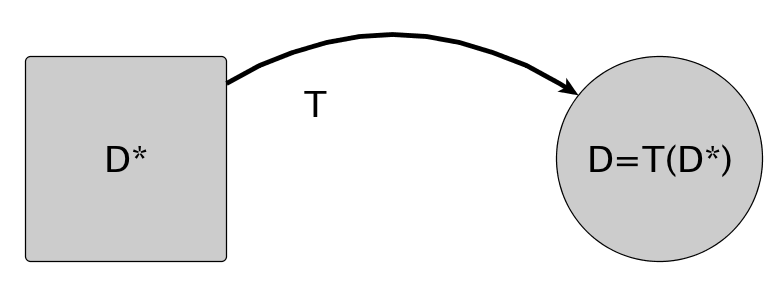
\includegraphics[scale=0.50]{CV.png}
	\end{center}
\end{teo}

\bibliographystyle{plain}
\bibliography{}
\end{document}
